
\chapter{Tutorial básico de uso do aplicativo Tracker}
\label{sec:tracker}
\vspace{-0.7cm}

Uma vez baixada a versão do aplicativo Tracker para o sistema operacional de seu computador, 
a partir do  endereço eletrônico  \href{https://physlets.org/tracker/}{\textcolor {blue}
{https://physlets.org/tracker/}}, instale-o seguindo as orientações no próprio sítio da Internet. Com o aplicativo instalado, siga os sete  passos descritos a seguir para realizar a tomada de dados.

\underline{\bf Passo 1:} {\bf Escolha de idioma português}\\
\vskip -0.5cm

Abra o aplicativo e no caminho Edit $>$ Language $>$ e escolha a opção português como mostra a Figura~\ref{fig1AppB}.

\underline{\bf Passo 2:} {\bf Abertura do arquivo do vídeo a ser analisado}\\
\vskip -0.5cm

Para abrir o arquivo do tipo vídeo  gravado com o celular faça um ``click'' na aba
``Arquivo'' e logo na aba ``Abrir''. Na janela que abrirá procure onde o arquivo   do tipo vídeo
está guardado e faça ``click'' nele. O Tracker carrega vídeos de quase todos os formatos gravados 
por celulares mas os arquivos não podem ser muito grandes (o arquivo carregado nas figuras 
deste tutorial era de 1,3 MB). Se o arquivo não abre tente reduzir o tamanho dele editando 
o vídeo no celular, cortando as partes em que a bolinha não se move, antes da queda, ou quando
já está no chão.
Na Figura~\ref{fig2AppB} vemos um vídeo já aberto para análise.
 \begin{minipage}{\linewidth}
      \centering
      \begin{minipage}{0.4\linewidth}
          \begin{figure}[H]
              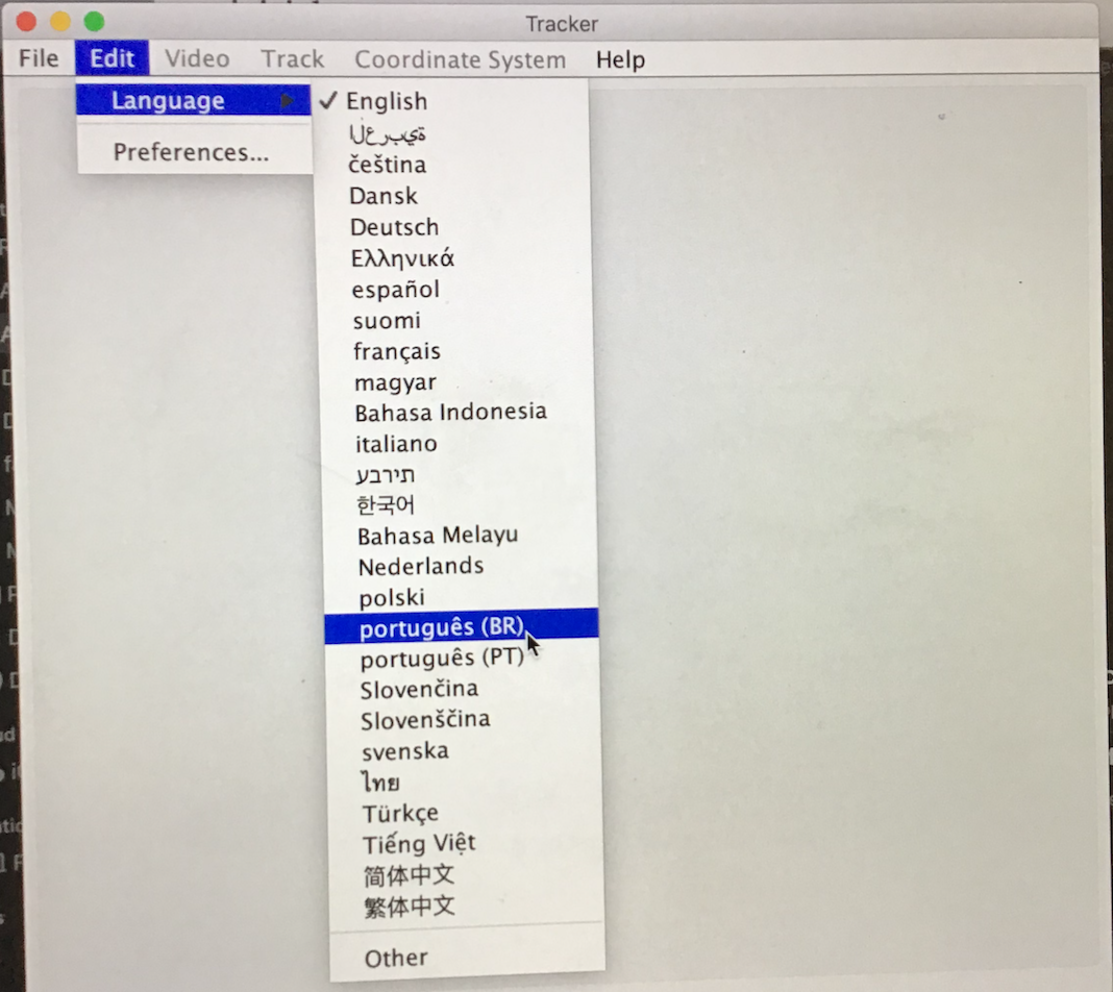
\includegraphics[width=\linewidth]{Figuras_exp3/fig1AppB.pdf}
              \caption{\label{fig1AppB} Escolha de idioma no aplicativo Tracker.}
          \end{figure}
      \end{minipage}
      \hspace{0.01\linewidth}
      \begin{minipage}{0.4\linewidth}
          \begin{figure}[H]
              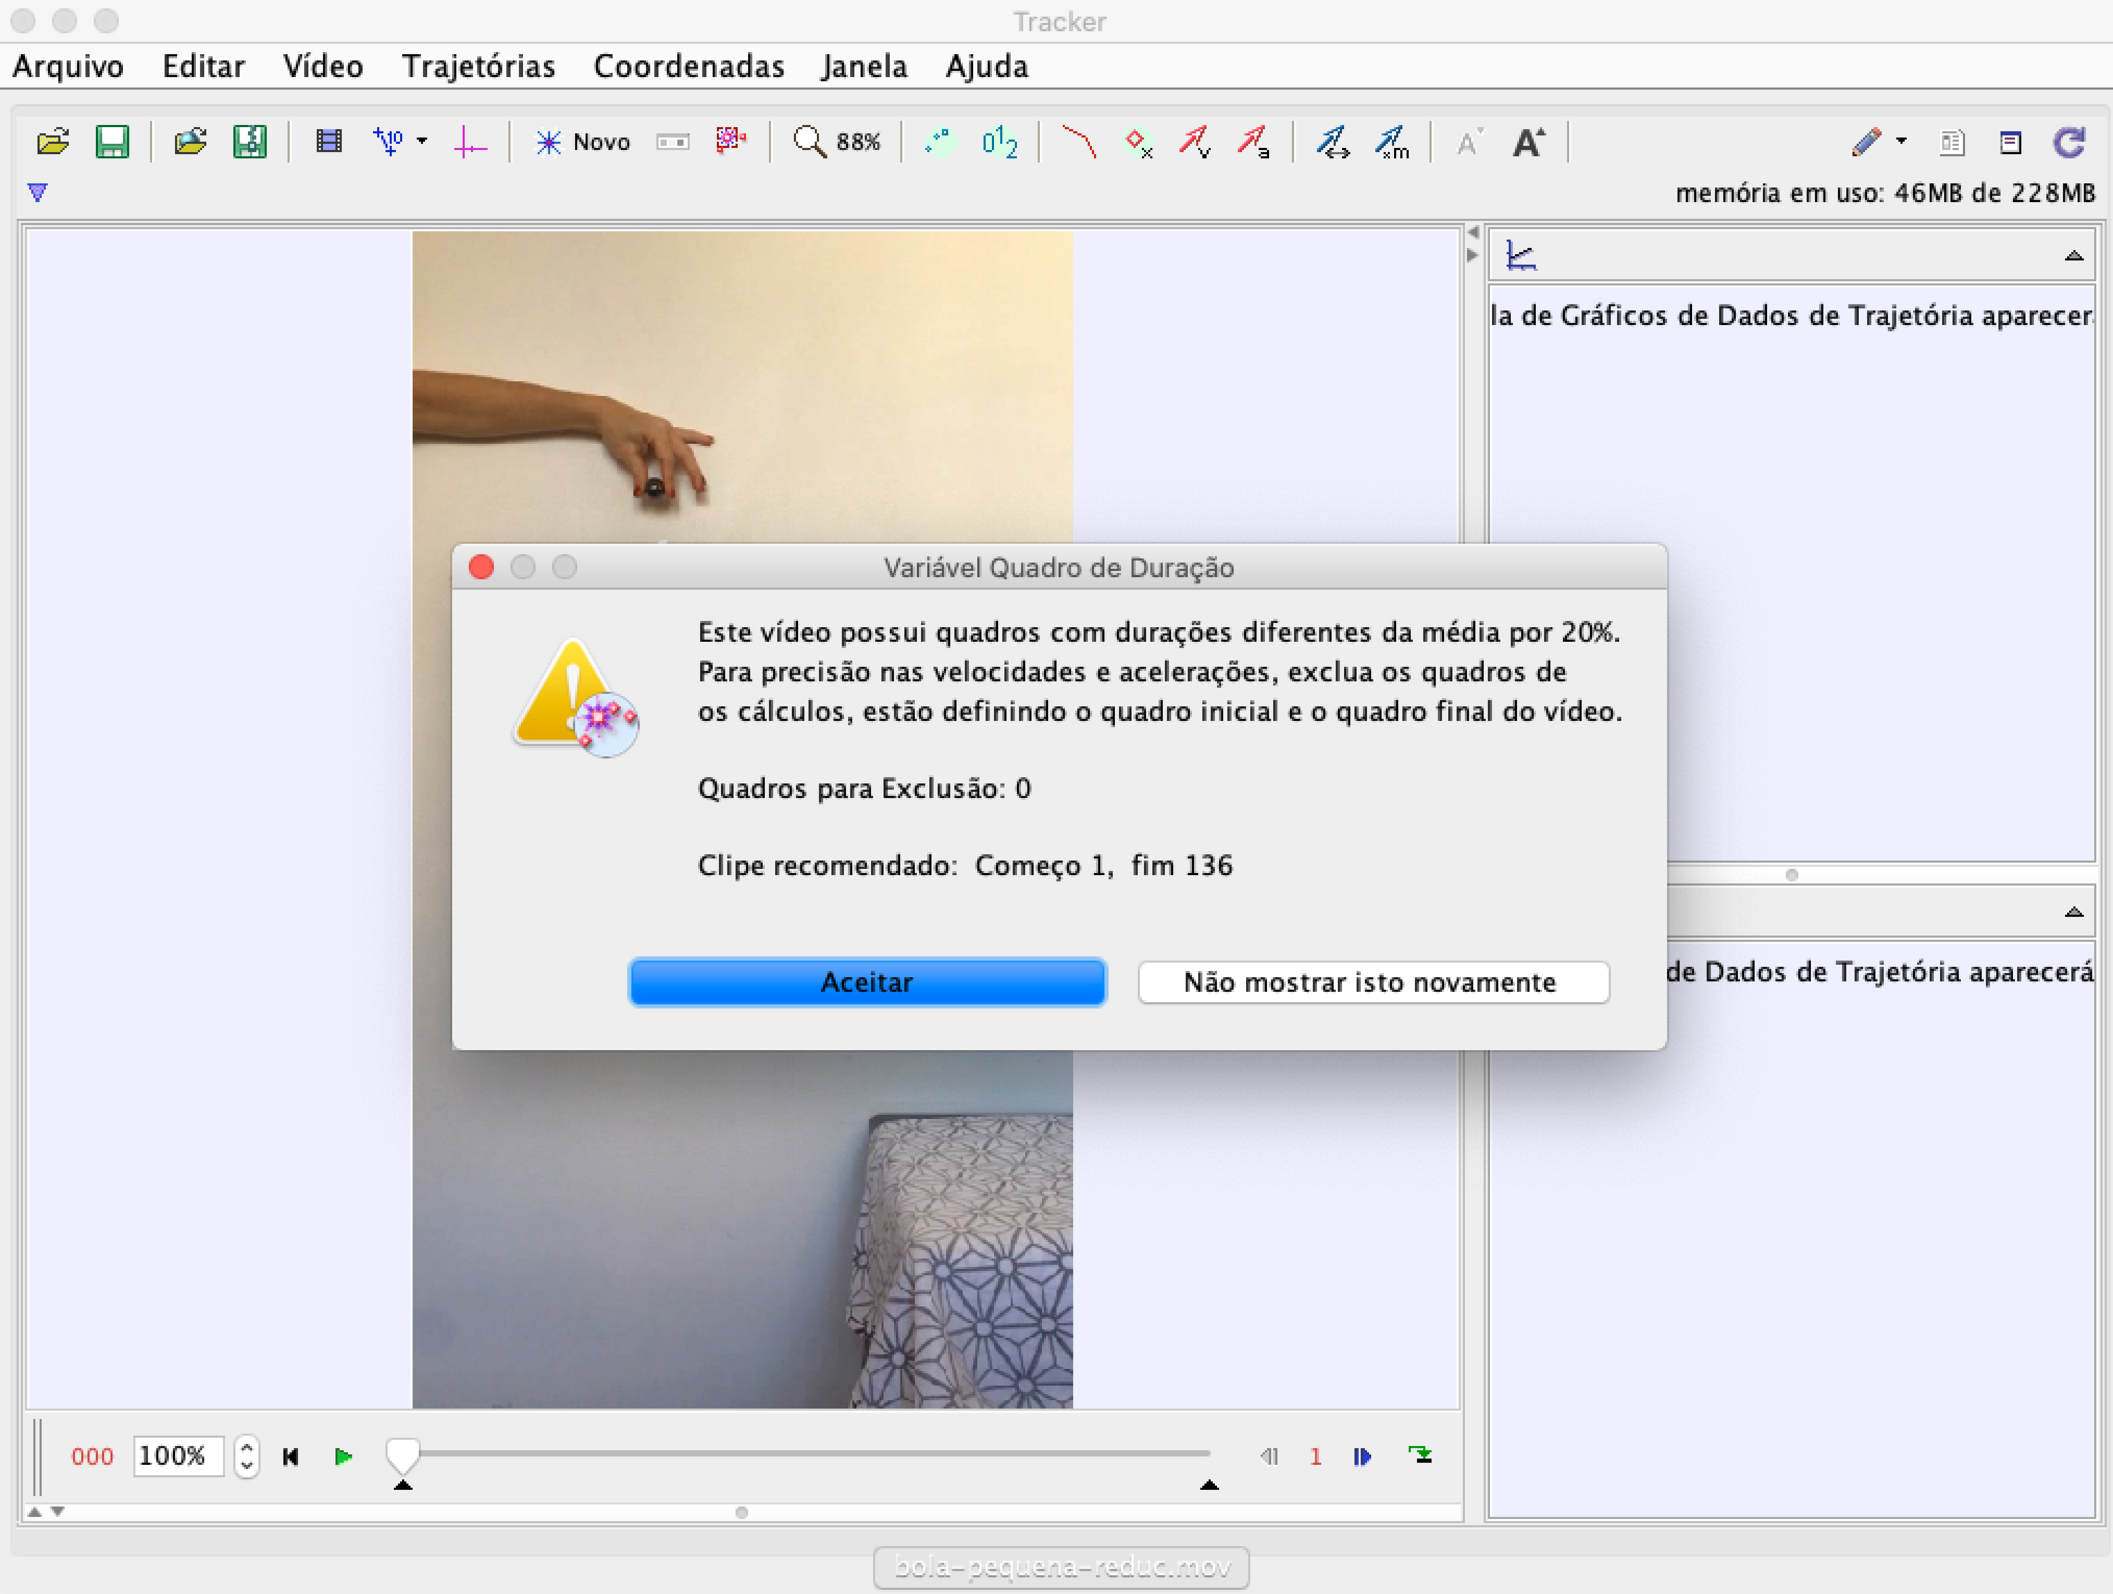
\includegraphics[width=\linewidth]{Figuras_exp3/fig2AppB.pdf}
             \caption{\label{fig2AppB} Ignore a mensagem na janela fazendo ``click em ``Aceitar''.}
          \end{figure}
      \end{minipage}
  \end{minipage}%

\underline{\bf Passo 3:} {\bf Determinação dos quadros inicial e final da análise}\\
\vskip -0.5cm

Faça ``click'' no ícone indicado pela seta preta na Figura~\ref{fig3AppB} para abrir a janela de 
``Ajustes de Corte de Vídeo''. Muitas vezes no lugar assinalado com uma seta vermelha na Figura
\ref{fig3AppB} aparece um valor muito próximo de $30.00/$s (trinta quadros por segundo), apague o valor e coloque exatamente  $30.00/$s.

As setas verdes e laranja da Figura~\ref{fig3AppB} mostram os lugares onde deveremos 
colocar os valores numéricos corretos dos quadros iniciais e finais respectivamente.
Para escolher o quadro inicial correto movimente o ícone preto indicado pela seta verde na Figura 
\ref{fig4AppB} até ver a bolinha justo saindo da mão. Verá que o valor numérico do quadro inicial 
se coloca automaticamente no lugar indicado pela seta verde na Figura~\ref{fig3AppB}. Para escolher 
o quadro final faça o mesmo com o ícone preto indicado pela seta laranja na  Figura~\ref{fig4AppB}. Escolha o quadro final mais o menos como no instante mostrado na  Figura~\ref{fig4AppB}.
Finalmente feche a janela ``Ajustes de Corte de Vídeo'' fazendo ``click em ``Aceitar''.

  \begin{minipage}{\linewidth}
  \centering
  \begin{minipage}{0.4\linewidth}
          \begin{figure}[H]
              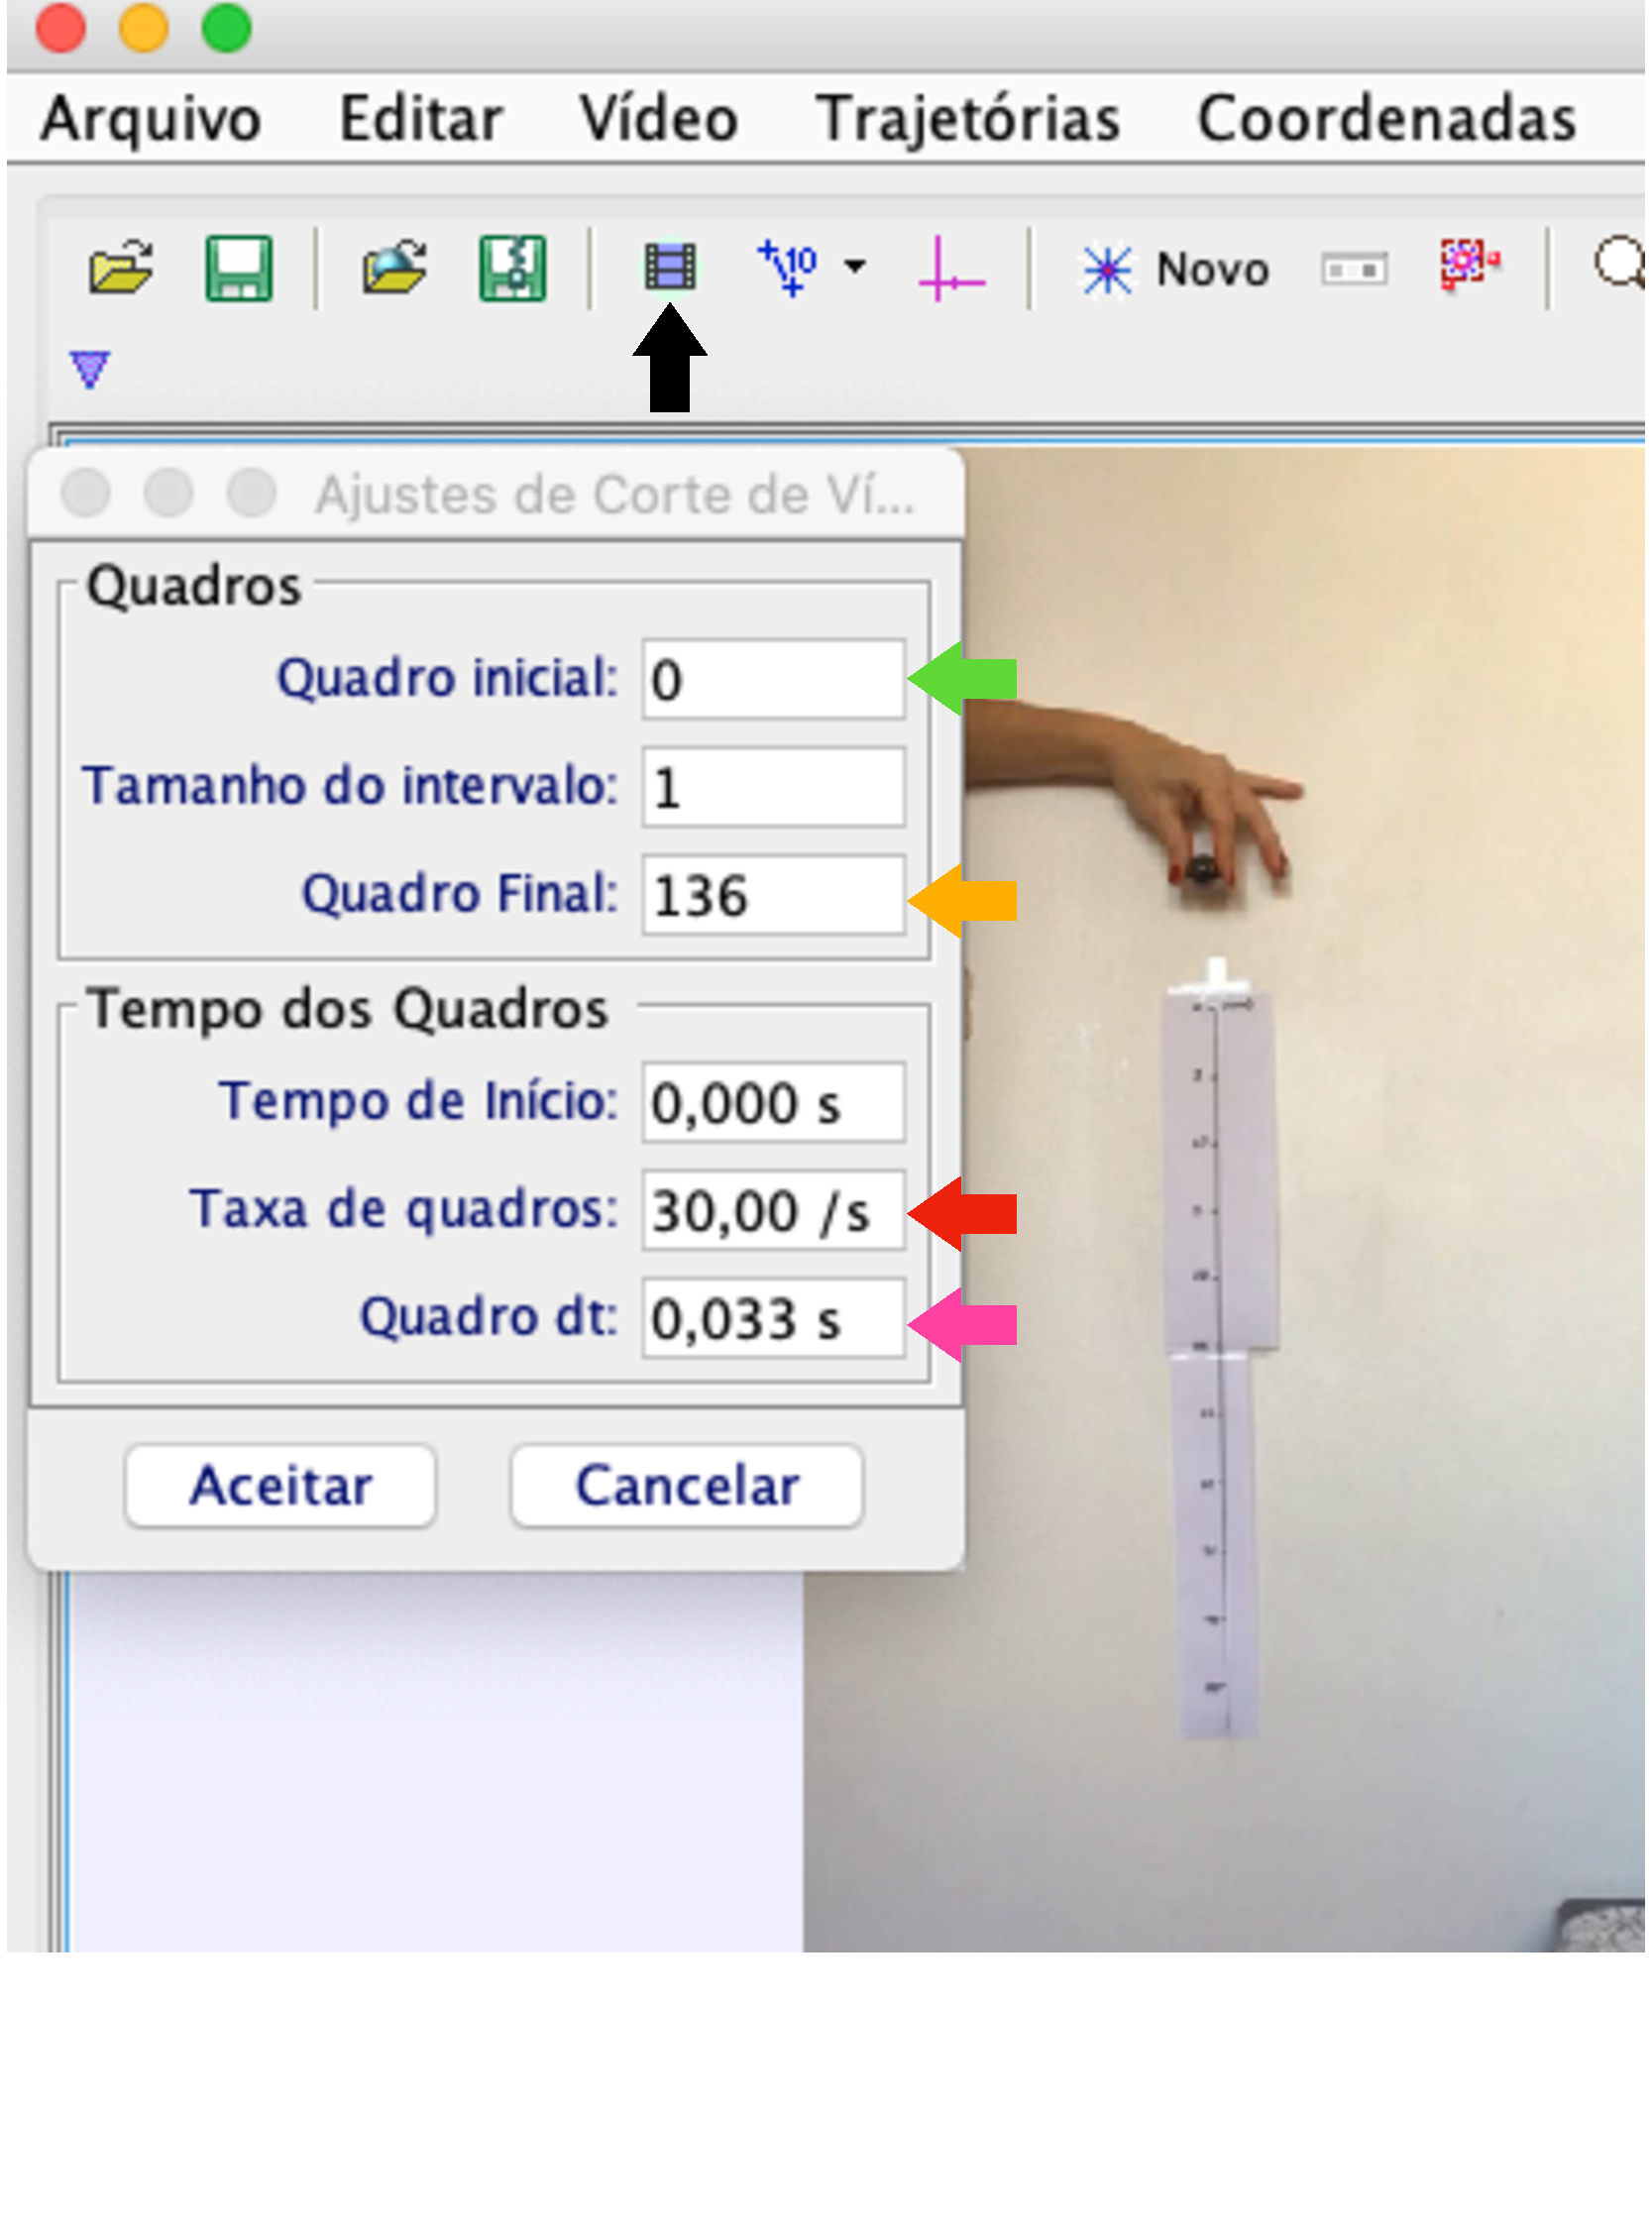
\includegraphics[width=\linewidth]{Figuras_exp3/fig3AppB.pdf}
\caption{\label{fig3AppB} Faça ``click'' no ícone indicado pela seta preta para abrir a janela de 
``Ajustes de Corte de Vídeo''.}
          \end{figure}
      \end{minipage}
      \hspace{0.01\linewidth}
      \begin{minipage}{0.43\linewidth}
          \begin{figure}[H]
              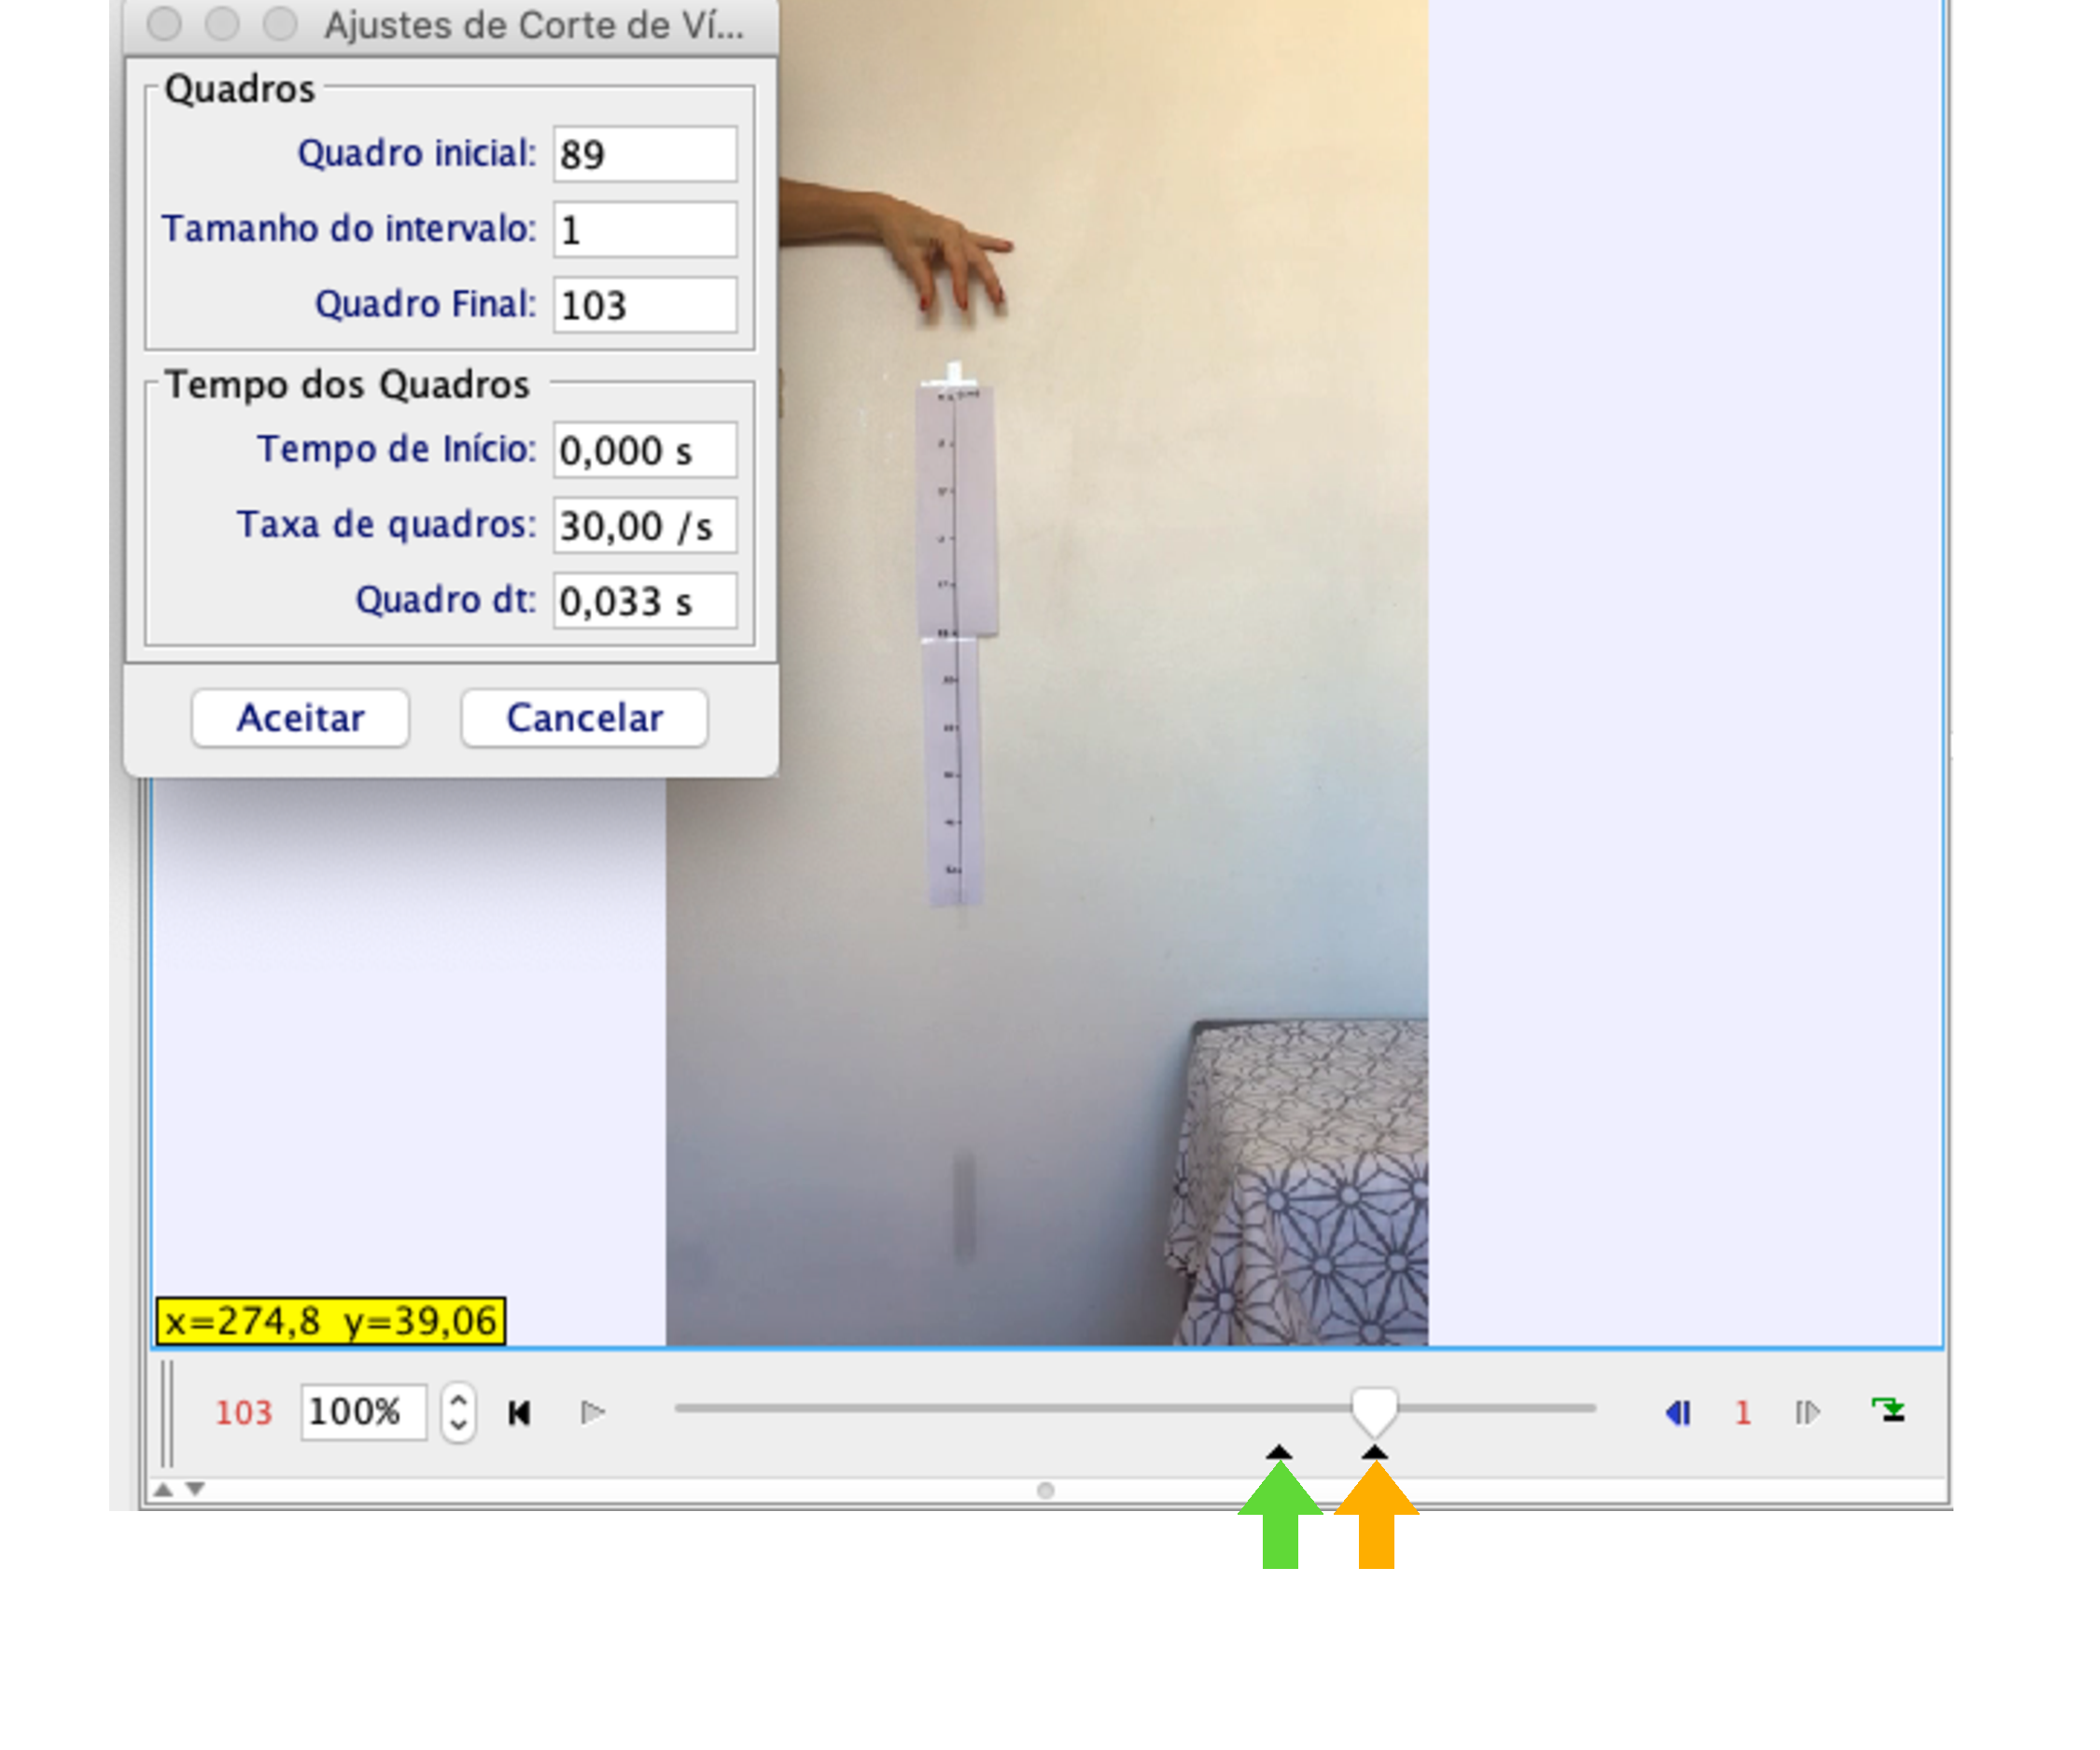
\includegraphics[width=\linewidth]{Figuras_exp3/fig4AppB.pdf}
\caption{\label{fig4AppB} Movimentando os ícones pretos indicados pelas setas verde e laranja escolhemos os quadros iniciais e finais respectivamente.}
          \end{figure}
      \end{minipage}
  \end{minipage}%

\underline{\bf Passo 4:} {\bf Escolha da escala de comprimentos}\\
\vskip -0.5cm

Faça ``click'' no ícone indicado pela seta preta  na Figura~\ref{fig5AppB} e escolha um novo 
``bastão de medição''. De um ``zoom'' na imagem escolhendo o aumento apropriado no ícone da lupa
de maneira de ver claramente a região da régua na imagem do quadro inicial.  
Mantendo apertada a tecla "shift" do computador selecione os pontos iniciais e finais sobre a régua
como indicado na Figura~\ref{fig6AppB}. Não esqueça de colocar na janela indicada nessa figura o valor real do comprimento do ``bastão de medição'' escolhido em metros.
  \begin{minipage}{\linewidth}
 \centering
      \begin{minipage}{0.35\linewidth}
          \begin{figure}[H]
              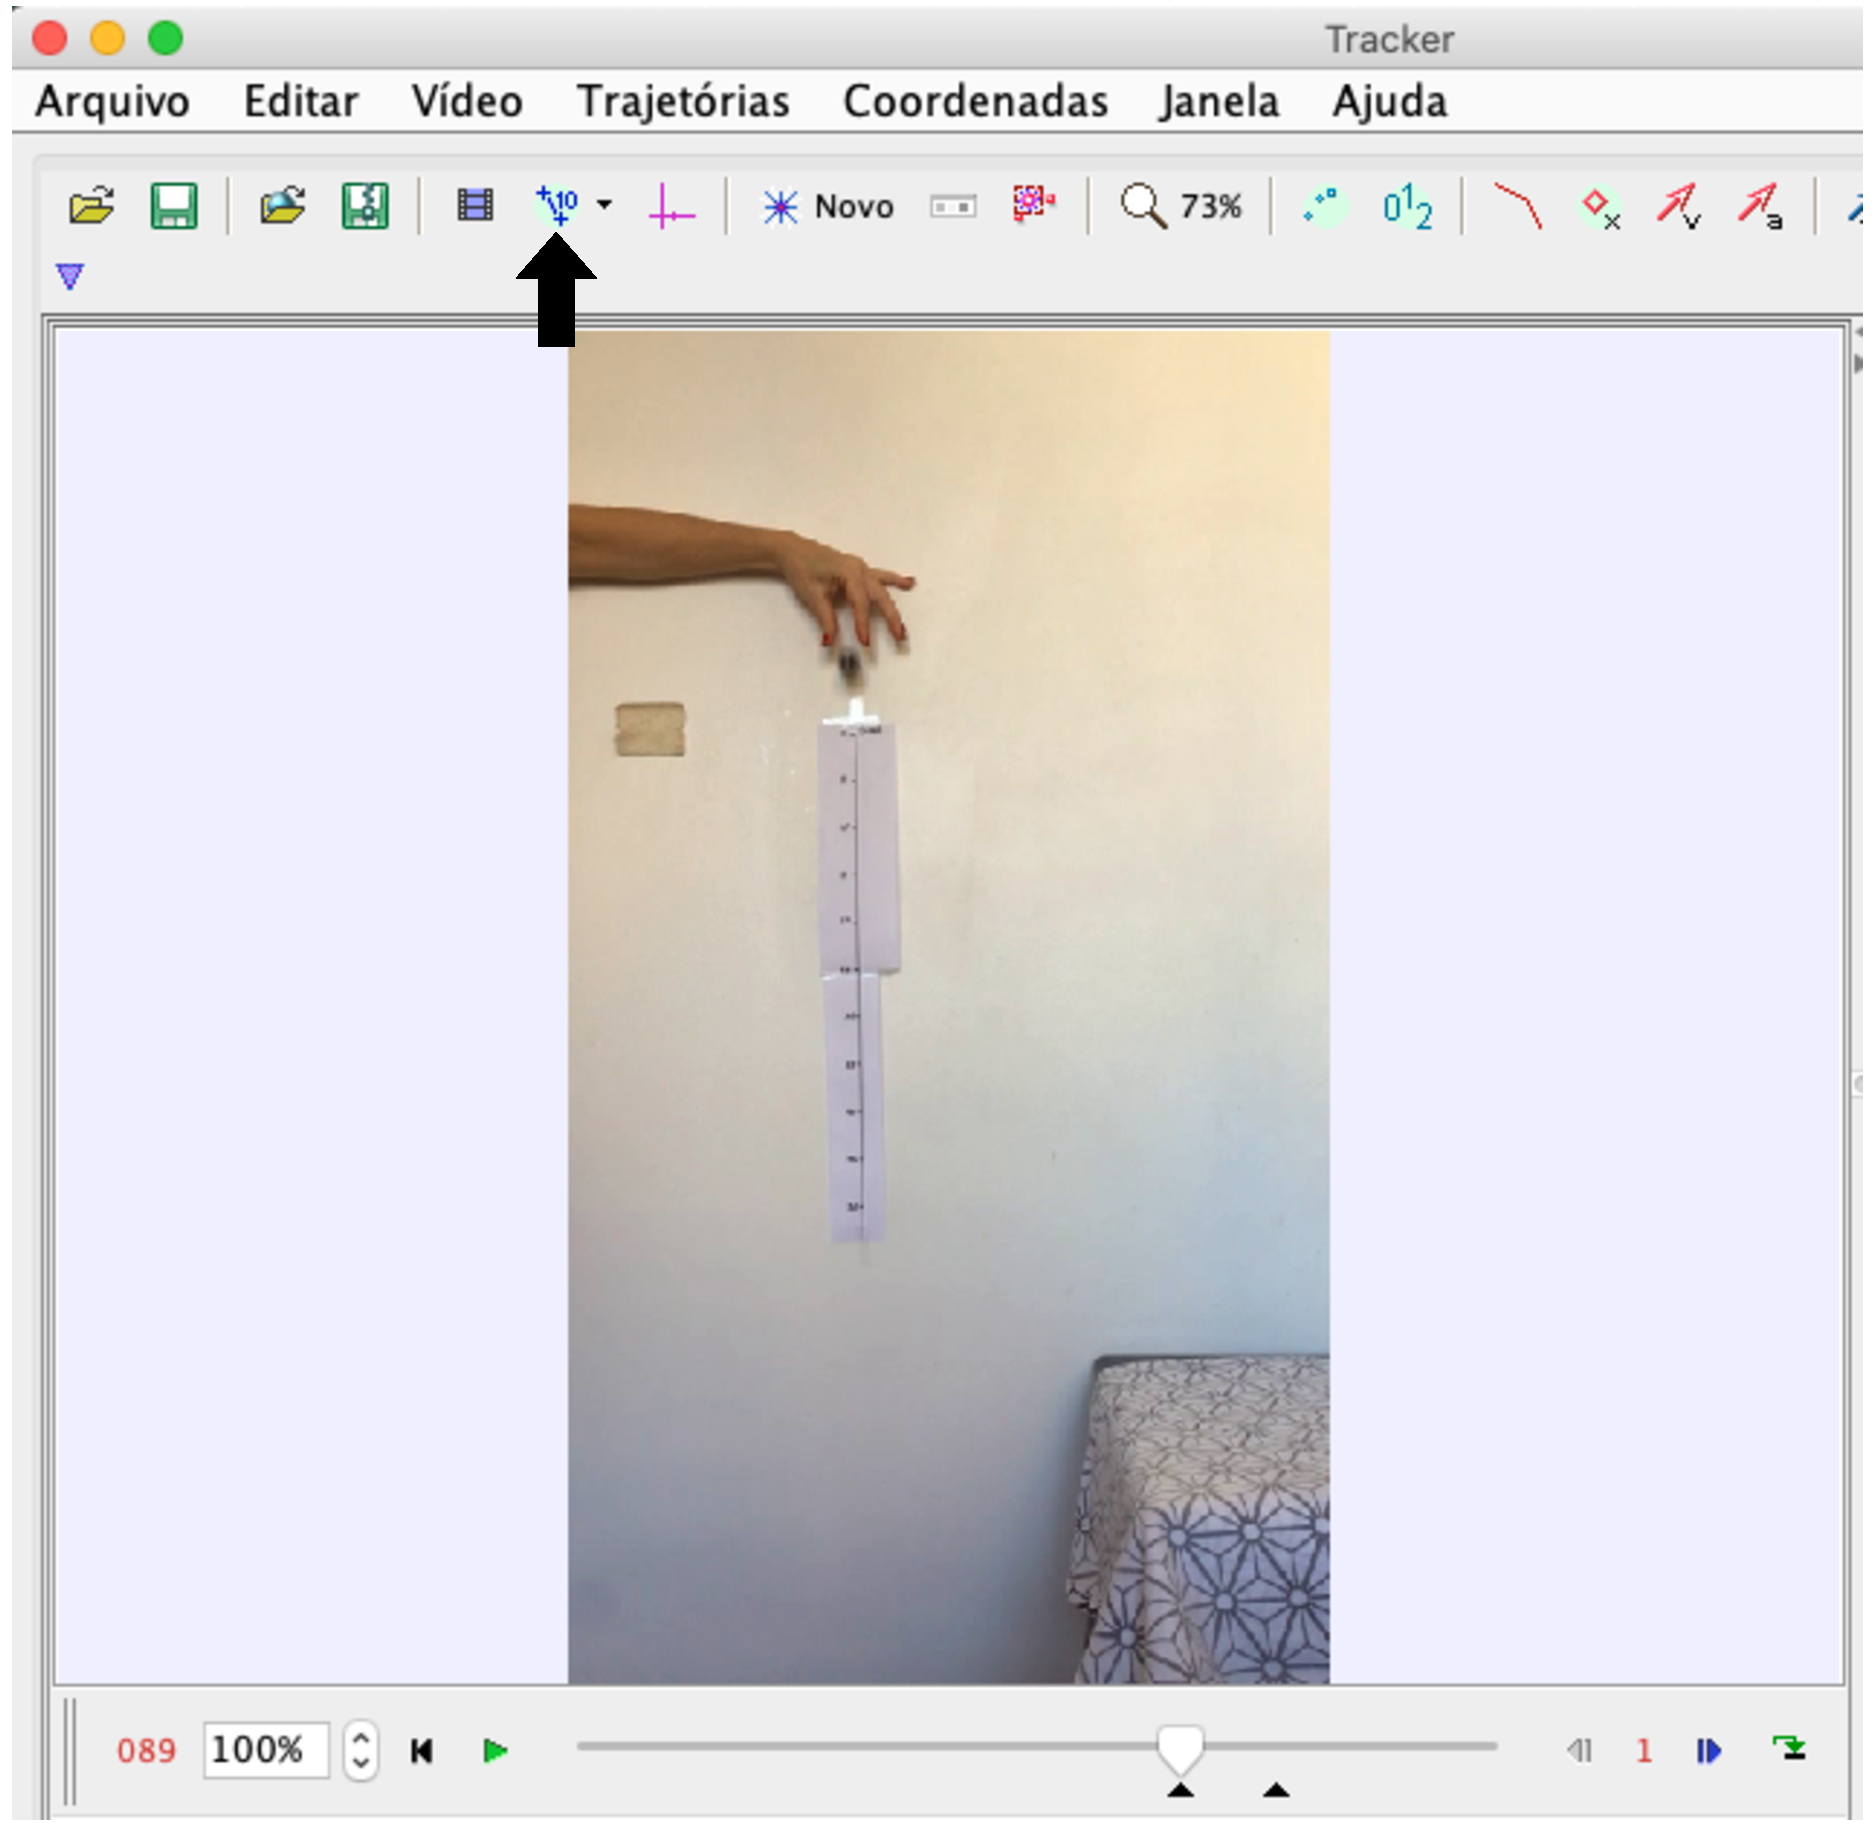
\includegraphics[width=\linewidth]{Figuras_exp3/fig5AppB.pdf}
\caption{\label{fig5AppB} Fazendo ``click no ícone indicado pela seta preta você pode escolher um ``bastão de medição'' que definirá a escala.}
          \end{figure}
      \end{minipage}
      \hspace{0.05\linewidth}
      \begin{minipage}{0.38\linewidth}
          \begin{figure}[H]
              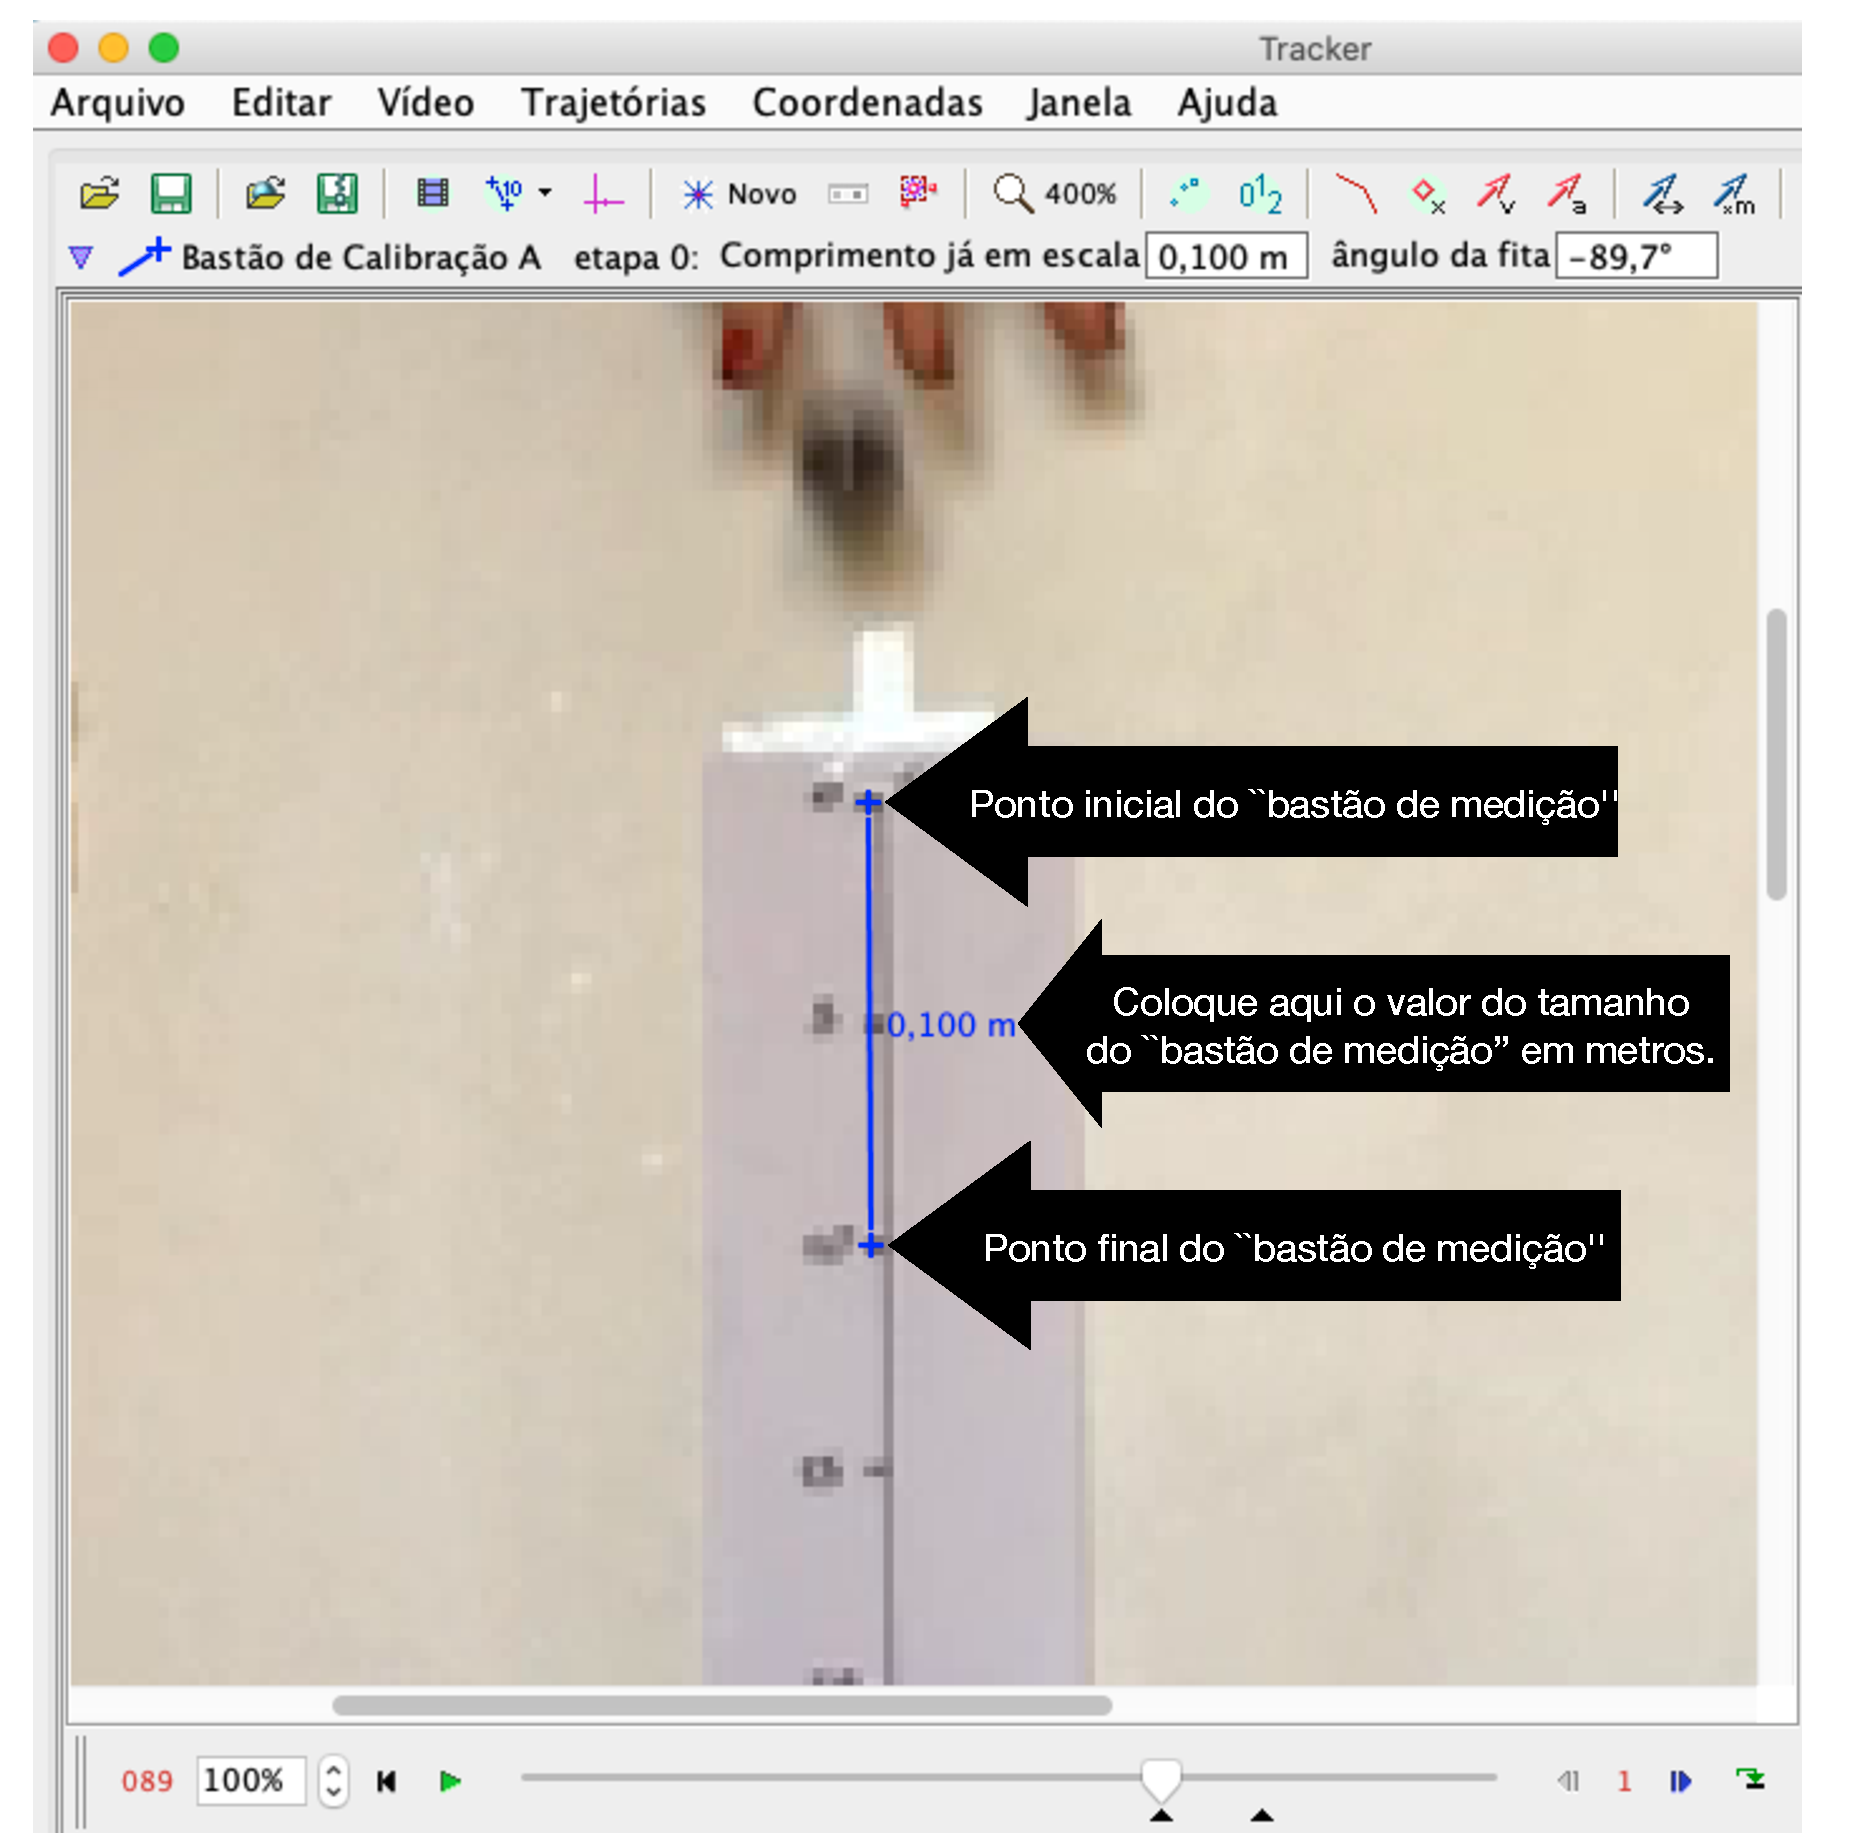
\includegraphics[width=\linewidth]{Figuras_exp3/fig6AppB.pdf}
\caption{\label{fig6AppB} Determinação do ''bastão de medição'' que estabelece a escala de comprimentos.}
          \end{figure}
      \end{minipage}
  \end{minipage}%


\underline{\bf Passo 5:} {\bf Escolha do sistema de coordenadas}\\
\vskip -0.5cm

Para escolher um sistema de eixos coordenados faça ``click'' no ícone indicado pela seta preta na Figura \ref{fig7AppB}. Dessa forma aparecerá o sistema de eixos cor de rosa da figura. Você pode deslocar 
a origem de coordenadas do sistema de eixos fazendo ``click'' com o botão esquerdo do mouse do computador e arrastando a origem para o local que você desejar. Também é possível inclinar o sistema de eixos se for necessário (nesta experiência não será necessário) fazendo ``click'' com o botão esquerdo do mouse do computador em qualquer eixo e arrastando esse eixo para obter a inclinação desejada.

\underline{\bf Passo 6:} {\bf Escolha da janela de controle da massa cuja trajetória
será determinada}\\
\vskip -0.5cm

Fazendo ``click'' no ícone marcado pela seta preta na Figura~\ref{fig8AppB} se abrirá a janela de controle 
 da massa (indicada pela seta vermelha  na Figura~\ref{fig8AppB}, cuja trajetória será determinada (neste caso a bolinha da figura). Fazendo ``click'' na seta verde você poderá escolher qual gráfico 
 quer visualizar uma vez escolhidos os pontos da trajetória cuja forma será ensinada no próximo passo deste tutorial.
Também fazendo ``click'' na aba ``Dados'' assinalada pela seta azul na  Figura~\ref{fig8AppB} se abrirá a janela onde você poderá selecionar (seta rosa na figura) as colunas que apareceram na janela de tabelas (indicada também na figura).
  \begin{minipage}{\linewidth}
      \centering
      \begin{minipage}{0.35\linewidth}
          \begin{figure}[H]
              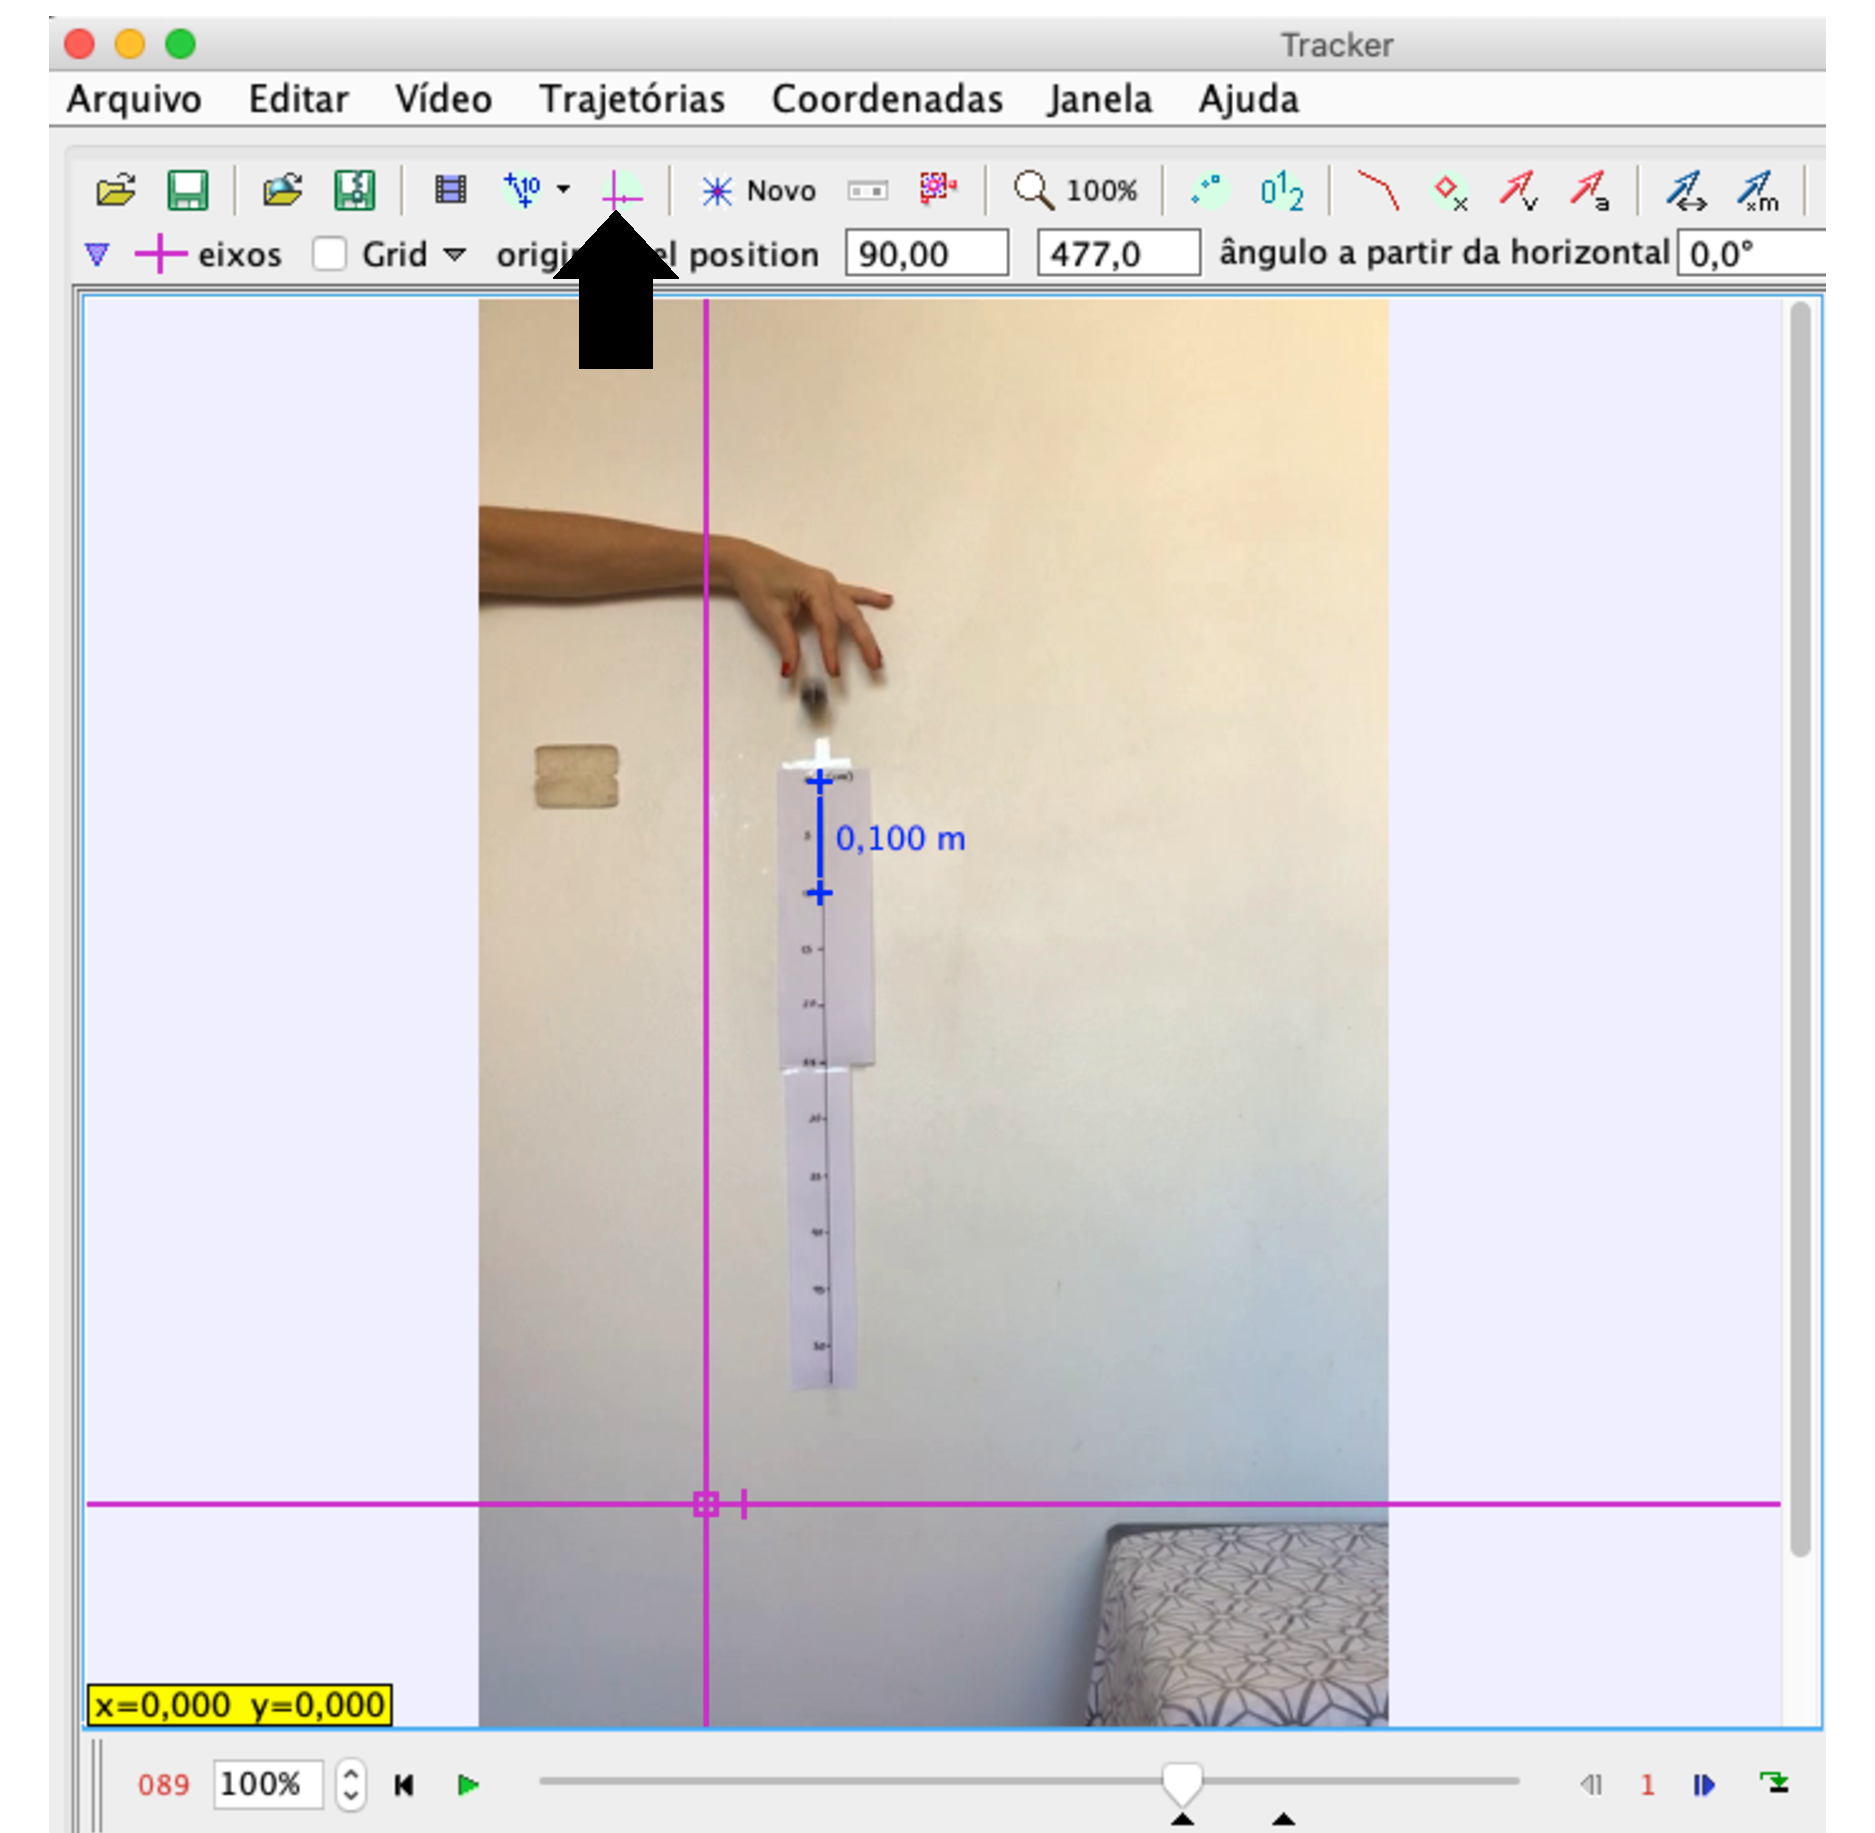
\includegraphics[width=\linewidth]{Figuras_exp3/fig7AppB.pdf}
\caption{\label{fig7AppB} Para criar um sistema de coordenadas (eixos de cor rosa na Figura) faça ``click'' no ícone indicado pela seta preta. Logo posicione a origem de coordenadas, como mostrado na figura, arrastando com o mouse do computador o quadrado rosa no sistema de eixos.}
          \end{figure}
      \end{minipage}
      \hspace{0.05\linewidth}
      \begin{minipage}{0.37\linewidth}
          \begin{figure}[H]
              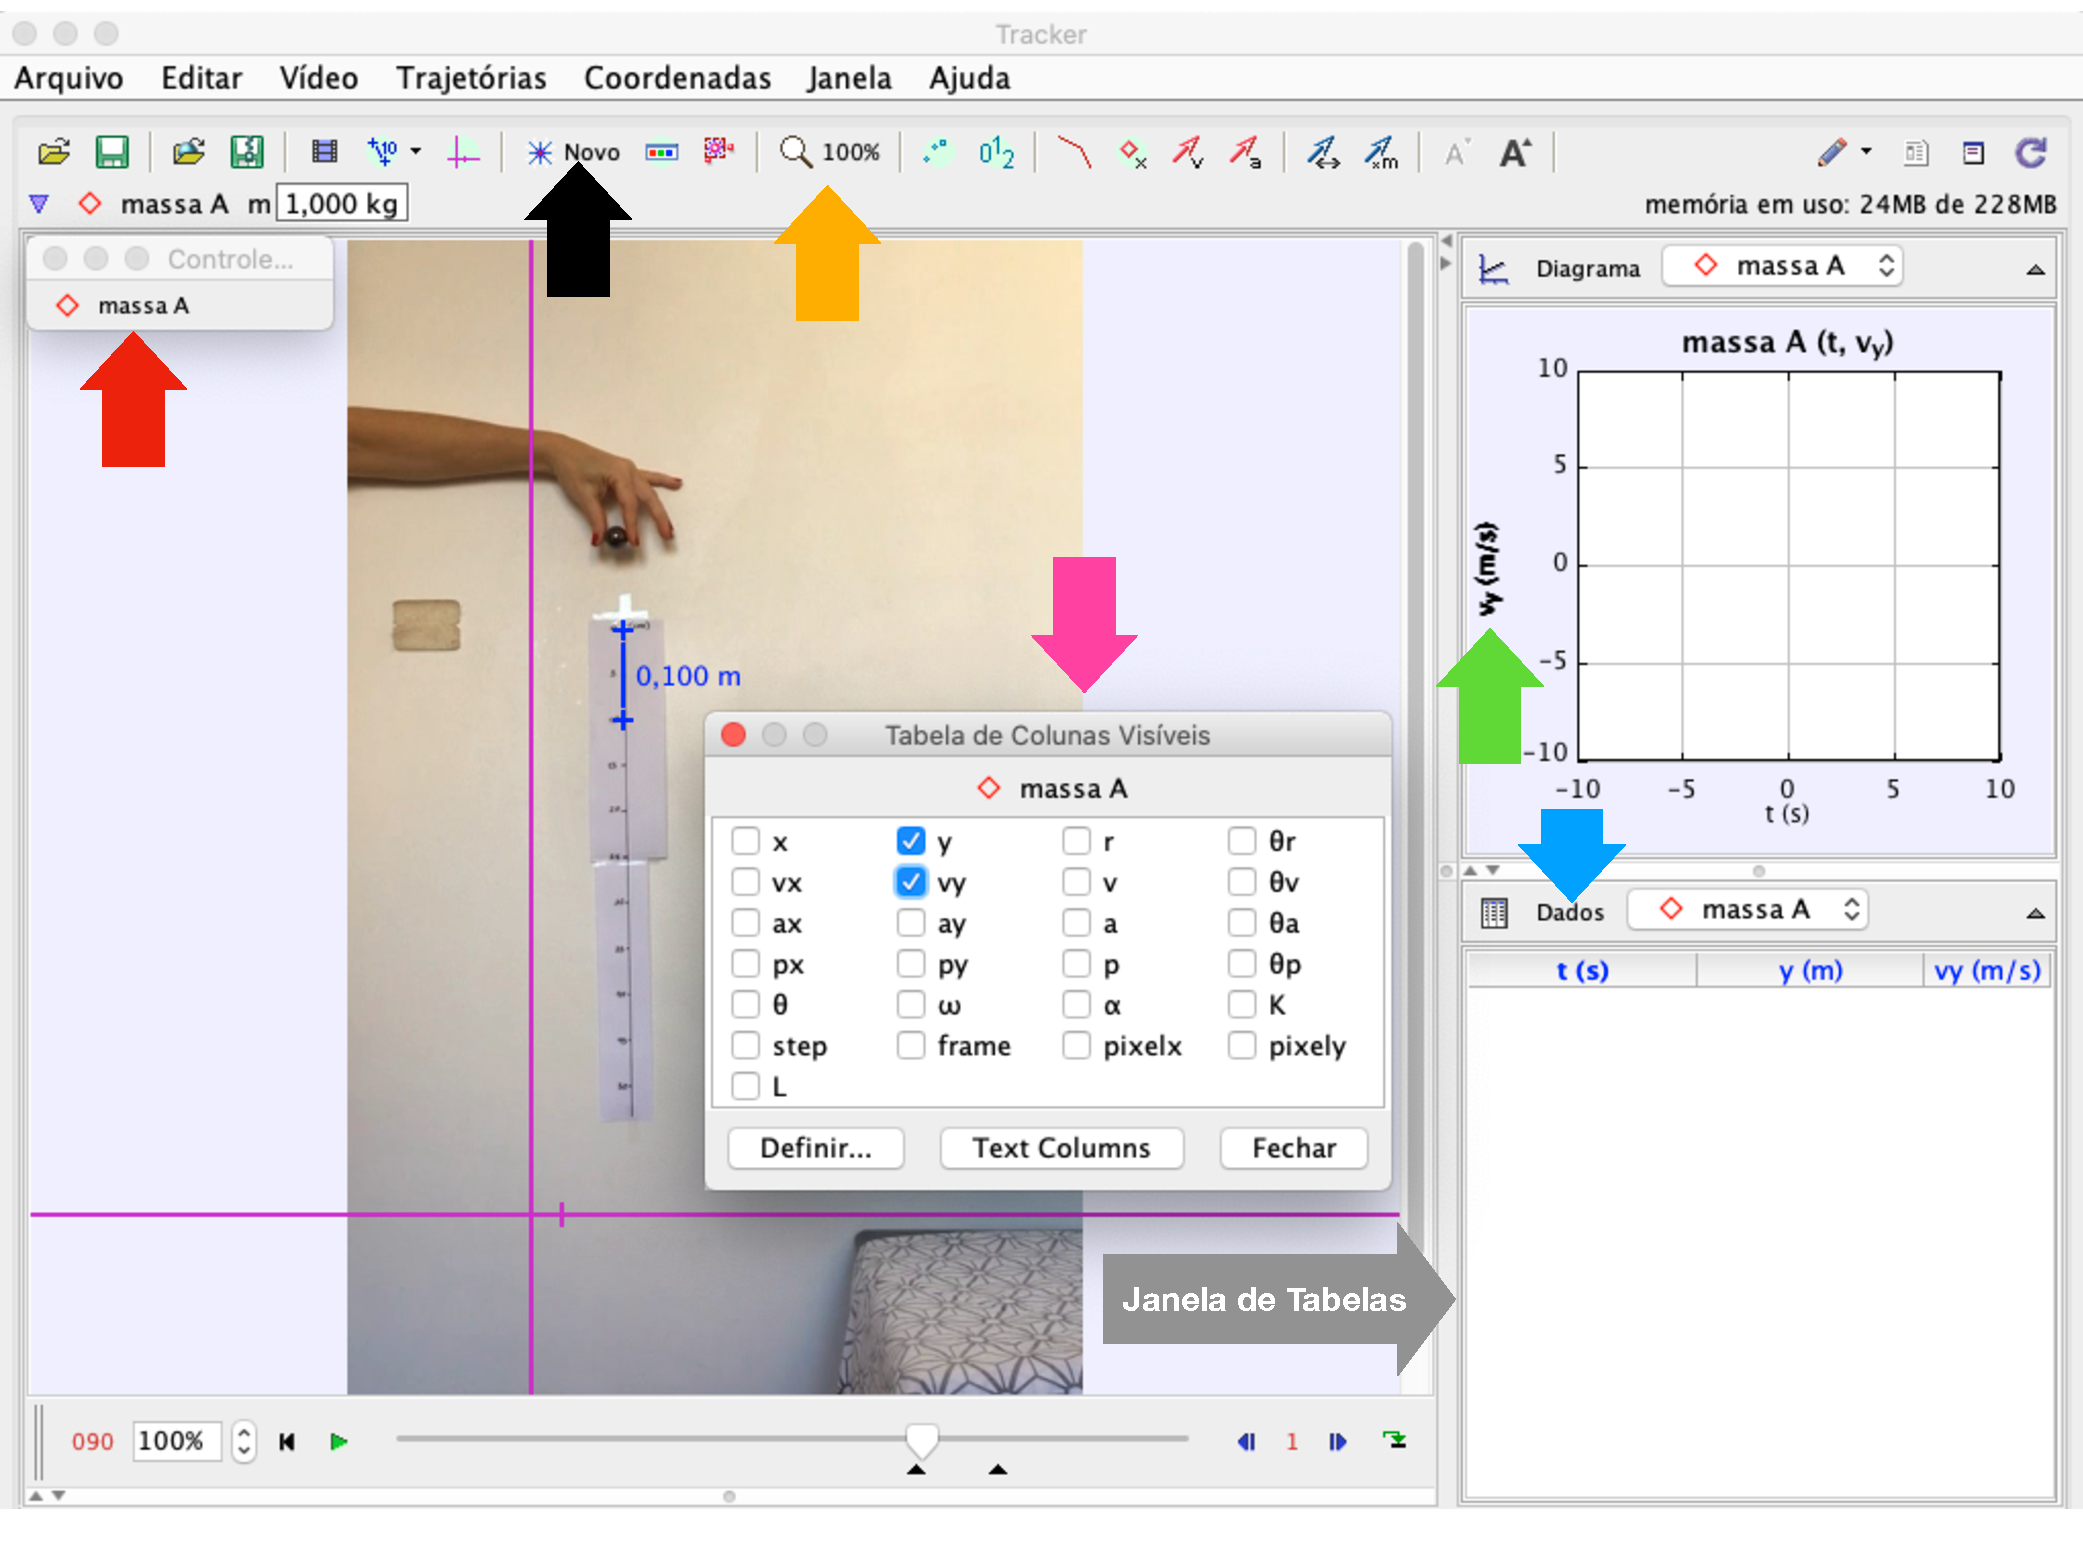
\includegraphics[width=\linewidth]{Figuras_exp3/fig8AppB.pdf}
\caption{\label{fig8AppB} Fazendo ``click'' no ícone indicado pela seta preta abre-se a janela indicada pela seta vermelha. Fazendo ``click'' no ícone indicado pela seta verde se escolhe o gráfico que quer ser visualizado 
após determinar os pontos da trajetória. Fazendo ``click'' na aba ``Dados'', indicada pela seta azul, 
abre-se a janela indicada pela seta rosa onde podem ser escolhidas as colunas das tabelas de dados que apareceram na janela de tabelas. Se precisar fazer um zoom na imagem pode usar a aba indicada pela seta laranja.}
          \end{figure}
      \end{minipage}
  \end{minipage}%
  
  
  
\underline{\bf Passo 7:} {\bf Determinação dos pontos da trajetória de uma partícula}\\


Para determinar os pontos da trajetória em forma manual você precisará manter 
apertada a tecla ``shift'' do computador durante todo o processo de medida . Ao apertar a tecla ``shift'' você entra no modo aquisição de dados e verá que o cursor virá um quadrado com um ``x'' no meio.
Ao fazer ``click'' no ponto que você quer traçar a trajetória (no nosso caso será o centro da bolinha)
pela primeira vez se marca um ponto da trajetória e a imagem pula automaticamente para o próximo quadro e ali você pode marcar o centro da bolinha novamente. Repita esse processo até marcar todos os pontos da trajetória contidos nas imagens entre os quadros iniciais e finais determinadas no passo 3 deste tutorial. À medida que você vai marcando os pontos da trajetória as colunas nas tabelas de dados (ver Figura~\ref{fig8AppB}) vão sendo preenchidas em forma automática.
\begin{figure}[h!]
      \centering
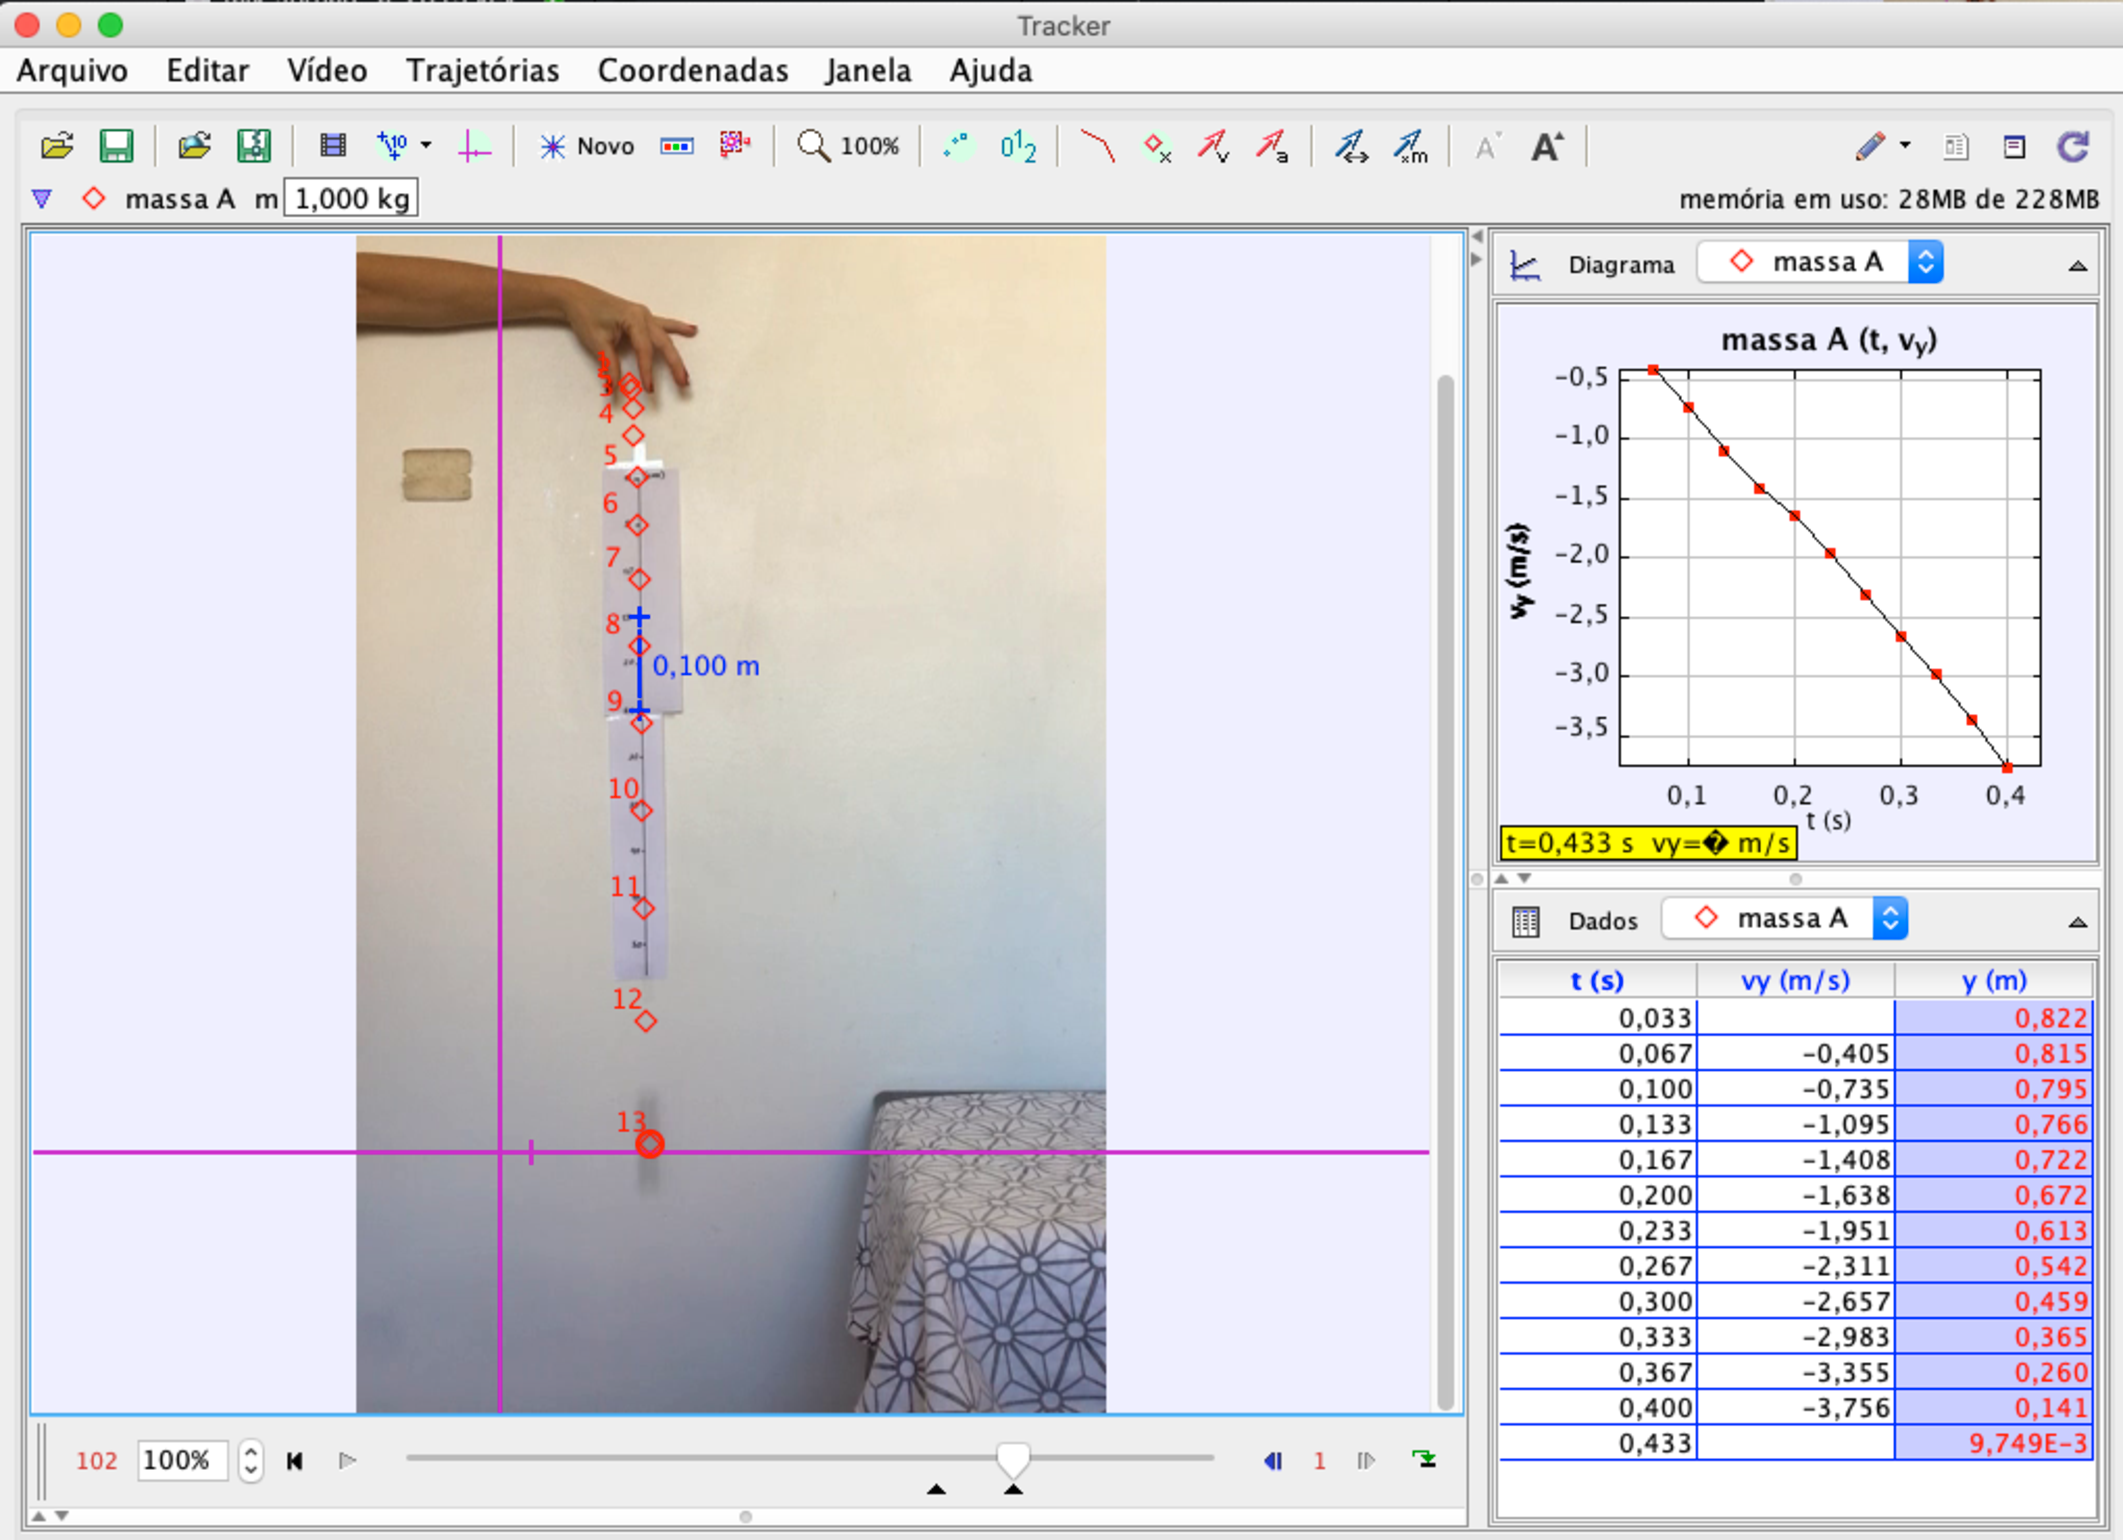
\includegraphics[width=9cm]{Figuras_exp3/fig9AppB.pdf}
\caption{\label{fig9AppB} Pontos da trajetória marcados e dados coletados nas colunas da janela de tabela.}
\end{figure}
No processo de medida é importante se auxiliar da ferramenta zoom, indicada pela seta laranja na 
Figura~\ref{fig8AppB}, para ter uma melhor imagem da bolinha e poder determinar com melhor precisão o seu centro. Uma vez escolhido um zoom (por exemplo $400\%$) para enquadrar a imagem 
da bolinha arraste a imagem com o mouse. Na Figura~\ref{fig9AppB} é mostrado 
o final do processo de medida. Fazendo ``double click'', com o botão esquerdo do mouse, no cabeçalho de uma coluna, na janela de tabela, você seleciona a janela e os valores ficaram da cor rosa como estão os valores da coordenada ``y'' na Figura~\ref{fig9AppB}. Uma vez selecionada a 
coluna, fazendo ``click'' com o botão direito do mouse você abrira uma janela com varias opções.
Na aba ``Números'' você poderá escolher o formato (sem com vírgula ou ponto para separar os decimais). Uma vez escolhido o formato você poderá copiar os dados selecionados para serem transferidos, por exemplo, para uma planilha tipo Excel. 
 